% version 1.00, date 10/10/16, auteur Kafui Atanley
Ce chapitre décrit les différents diagrammes d'intéraction.

\section{Fonctionnalité 8}
Ce paragraphe décrit le diagramme d'intéraction concernant la fonctionnalité 8 soit la géolocalisation. \\

La figure suivant (figure \ref{diagrammeInteraction1}) indique le déroulement de la consultation d'une entité possédant une adresse.
\begin{figure}[H]
	\centering
	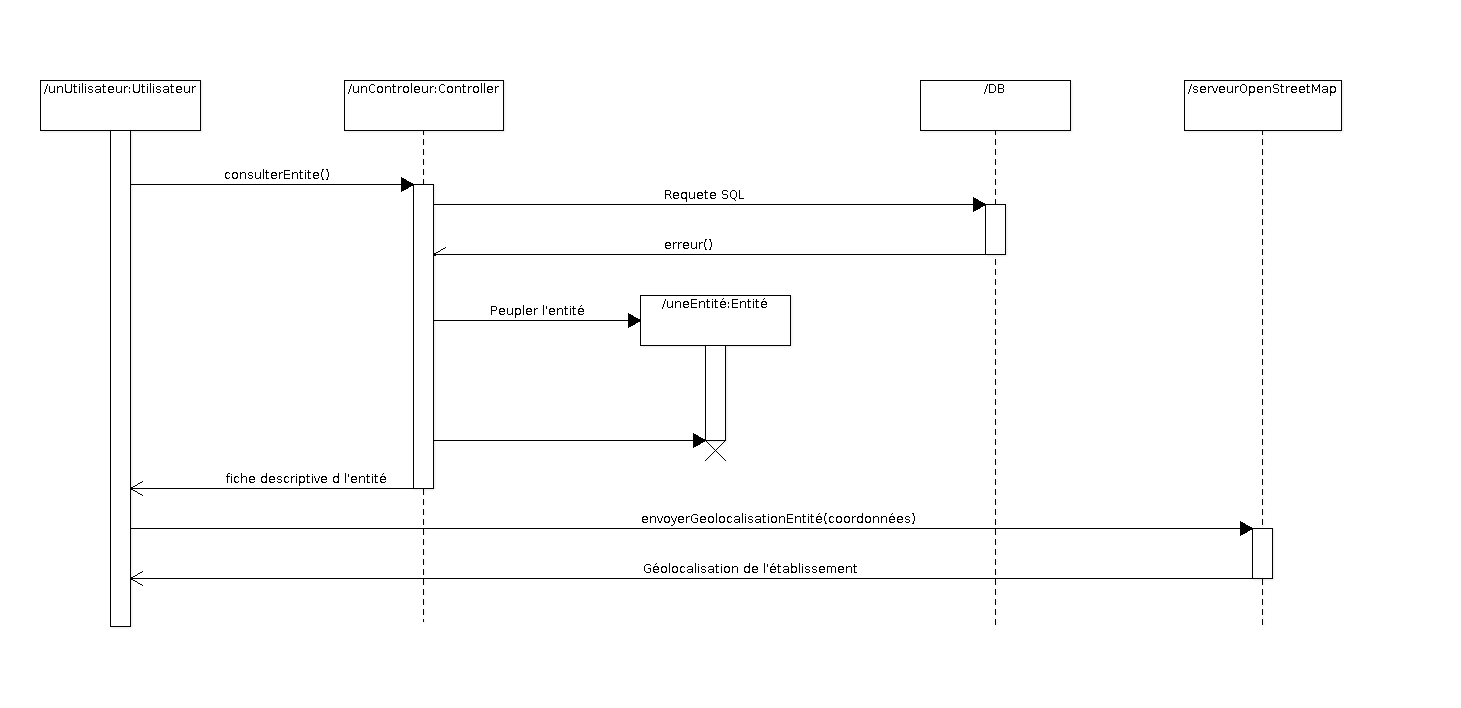
\includegraphics[scale=0.39]{images/diagrammesInteraction/01_diagrammeInteractionF8.png}
	\caption{Diagramme d'intéraction~: consultation d'une entité possédant une adresse}
	\label{diagrammeInteraction1}
\end{figure}

\section{Fonctionnalité 9}
Ce paragraphe décrit le diagramme d'intéraction concernant la fonctionnalité 9 soit l'attribution de frimousse. \\

La figure suivante (figure \ref{diagrammeInteraction3}) indique le déroulement de l'attribution d'une intervention de type frimousse.
\begin{figure}[H]
	\centering
	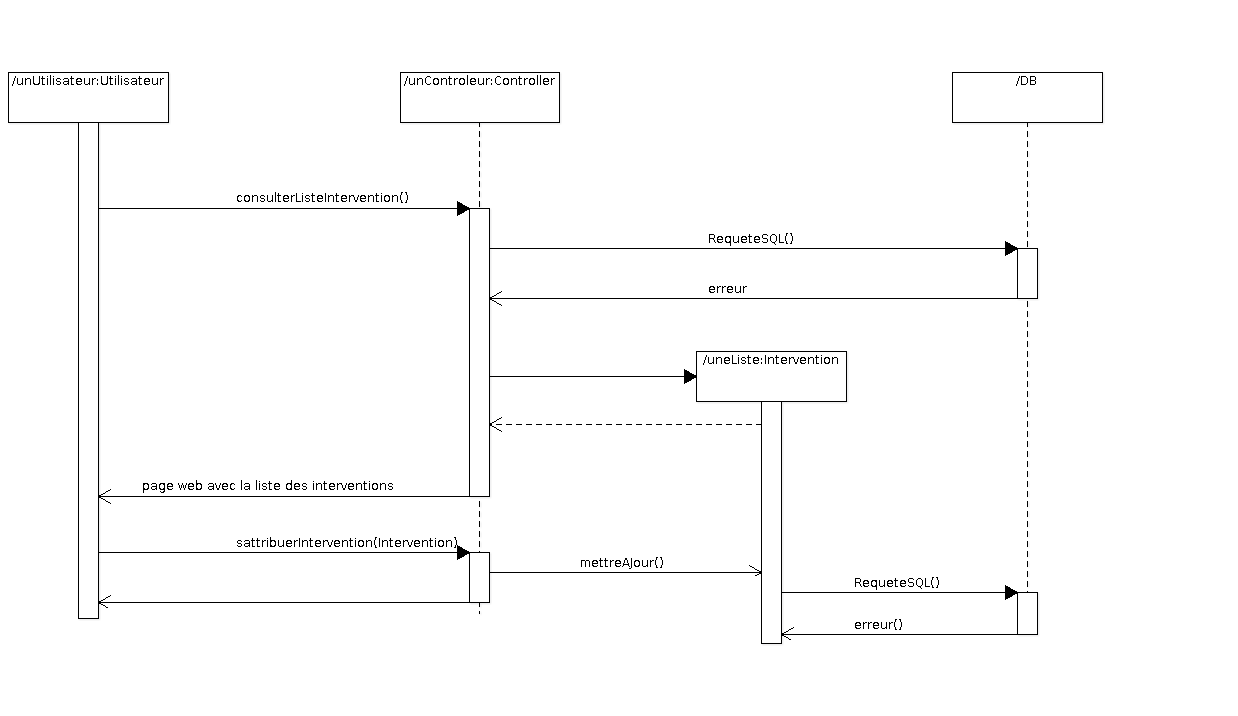
\includegraphics[scale=0.45]{images/diagrammesInteraction/02_diagrammeInteractionF9.png}
	\caption{Diagramme d'intéraction~: attribution d'une intervention de type frimousse }
	\label{diagrammeInteraction3}
\end{figure}

\section{Fonctionnalité 10}
Ce paragraphe décrit le diagramme d'intéraction concernant la fonctionnalité 10 soit la gestion des ventes. \\

La figure suivante (figure \ref{diagrammeInteraction3}) indique le déroulement de la création, modification, suppression d’une vente par un utilisateur. Il est à noter que seules les administrateurs auront la possibilité de supprimer une vente.
\begin{figure}[H]
	\centering
	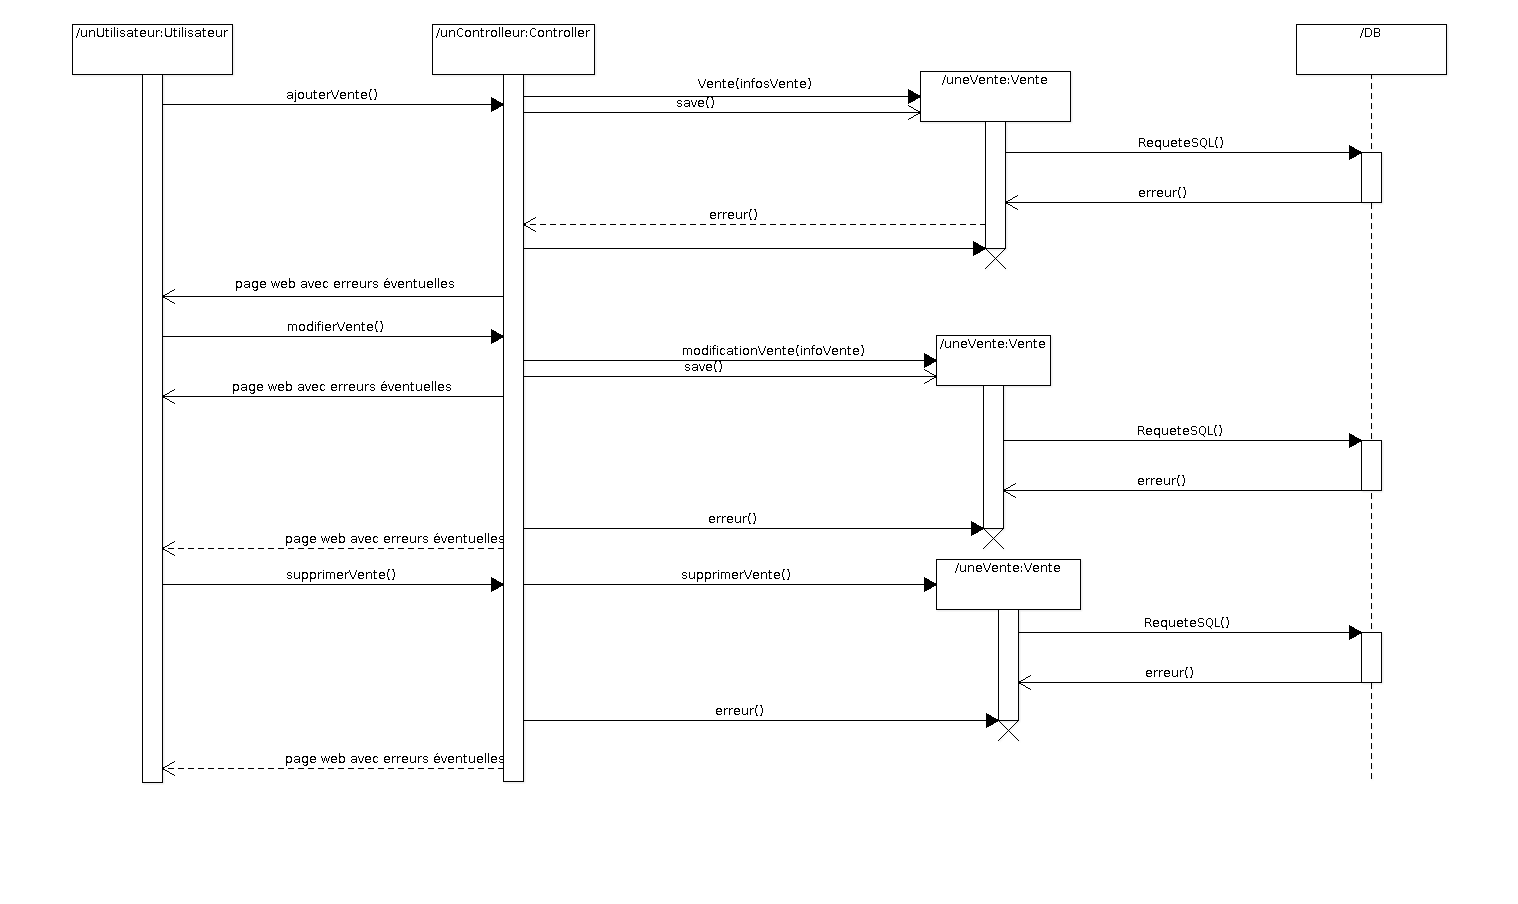
\includegraphics[scale=0.35]{images/diagrammesInteraction/03_diagrammeInteractionF10.png}
	\caption{Diagramme d'intéraction~: Création, modification, suppression d’une vente par un utilisateur}
	\label{diagrammeInteraction3}
\end{figure}



